\documentclass[11pt]{article}

\usepackage{amsmath}
\usepackage{amssymb}
\usepackage{cite}
\usepackage{hyperref}
\usepackage{graphicx}

\newcommand{\shellcmd}[1]{\\\indent\indent\texttt{\footnotesize\# #1}\\}

% Add bibliography style in the brackets below.
%\bibliographystyle{}

% The title text is entered in the brackets below
\title{An Interactive CBR System (AICS)}

% Author names are listed here.
\author{
  Betanzos, Miguel\\
  \texttt{gaurwraith@gmail.com}
  \and
  Blanco, Guillem\\
  \texttt{gblanco92@gmail.com}
  \and
  Moreno, Jonathan\\
  \texttt{jmoreno@lsi.upc.edu}
}
\date{}

\begin{document}
\maketitle


\section{Introduction}

This document outlines the main aspects of the developmentn of An Interactive CBR System (\emph{AICS}).

This CBR system aims to be an interactive system that the user can manage step by step. This project is open-ended as it exposes the infrastructure and few specific features are provided. We do this in order to be as general as possible, this way the user can implement its own method to deal with the peculiarities of their problems. While many options can be configured via the input console, the inner structure of our CBR is intended to facilitate the addition of features that can further expand the system.

\section{Implementation details}

We want to remark that one of the pros of this implementation is how it is structured. It maintains a modular structures allowing its extension. For example, if a new similarity distance for real values is needed we only have to add such similarity distance in the class Attributes, specifically into the \emph{RealAttr} class. This programming approach is applied along all the CBR tool implementation.

As we can see in the guided example (see the User Manual document), we allow to the user to load any csv that have a dataset being the CBR the one that adapts to the dataset once it knows the order of the attributes. It is not limited neither by the number of attributes nor its nature.

\subsection{Case structure}

A case in our system is represented as a hash map between the attribute names and the information contained in an attribute. This way the case structure can be general enough to hold any kind of attribute. A single case also holds a solution (label) that is also a hash map. This allows the user to encode anything as a solution: real/categorical value, a multi-label problem or even setting as label all the attributes which can be useful in recommendation systems. A case also holds some meta data about its utility and its evaluation in terms of decide which label is the solution for a new case introduced to the system.

A single attribute has its own type that encapsulates the information about itself together with a similarity function. This way real attributes that contain real values but have different similarities have a different type. This first version of AICS ships with the following attribute types: \texttt{RealAttribute}, \texttt{CategoricalAttribute}, \texttt{StringAttribute}. The user can expand the system by adding more attribute types that fit its needs.

\subsection{Library structure}

We have implemented two types of library structure: a flat memory and a hierarchical memory. The first one is a contiguous memory representation of the cases. The second uses a $k$-d tree to make a hierarchical representation of the cases. The $k$-d tree uses inter-quantile spread as attribute selection method. However, $k$-d tree can not handle categorical attributes. To fix this problem we have decided to split only real attributes and when we cannot split further we leave batches of instances in the labels. This way if the data set has only real attributes we get the usual $k$-d tree and if the data set has only categorical attributes we get a flat memory representation. How to retrieve from this kind of $k$-d tree is explained in the next section.

\subsection{Retrieval}

The retrieval phase in the flat memory case is pretty straightforward. We need to compute the similarity between the new case and all the cases stored in memory. This requires iterating over all the stored instance and can be computationally expensive if the number of instances is large. Hierarchical memory representation solves this problem partially by using a $k$-d tree in which retrieval can be done in $\log n$ operations (where $n$ is the number of stored instances). 

In the case where we have a mixture of real and non real data we can retrieve in the $k$-d tree by traversing the tree using only the real attributes. The tree then returns a batch of instance and we can do a linear iteration over the returned instances to find the ones with lower similarity (being the number of returned instances much lower than the total number of instances).

\subsection{Similarities}
As we have seen, the similarity calculation between the cases stored in memory and the new case introduced by the user is done by means of the attributes encapsulated in the case class. Since a case may be composed by attributes of different nature, that might need different similarity measures, these measures are calculated locally at each attribute. 

Hence we compute a straightforward Euclidean distance for real valued attributes, normalized to return a value between 0 and 1, being 0 the most similarity possible and 1 the most dissimilarity possible. The total similarity for a given case is the sum of each of its attributes' similarity. Furthermore, we can set different weights to each attribute independently in those cases that some attributes are more important than others. 

In the case of categorical attributes, the similarity is just checking whether the two of them are an exact match or not, a Boolean indicating exact match with 0 and no match with 1.

For the case of strings we have implemented a function that measures the Jarow-Winkler distance between two strings. This distance takes into account string length, character matches, position of the matching character, and several permutations of the string characters.

The structure of the attributes and cases makes it quite easy to add different similarity measures to existing attribute types, so, for instance, using cosine distance or other desired distance measure, just implies building it into a simple function and calling it from within the attributes.


\subsection{Adaptation}
For the adaptation phase, first of all we collect as many cases as we have specified to the retrieval tool. Then, from this set of cases that are similar to the new case proposed, if there is a consensus, that is, if all retrieved cases possess the same class label, we conclude that the new case is also of that class. 

When there are several classes to choose from, we implemented an approach that takes into account the utility and evaluation of the retrieved cases.

Each cases have assigned an utility and an evaluation. A high utility means that such case have been useful lots of times and consequently, the solution that it proposes have more relevance. The evaluation says if the cases is well resolved since we can have stored at memory wrong-classified instances.

Hence, our approach relies into a punctuation system. For each of the retrieved cases we give some punctuation for the solution that it proposes. This punctuation is weighted proporcionally to the utility. Moreover, this punctuation could be positive or negative depending if the case is well or wrong classified. For example, we can have one wrong-classified similar case with high utility. This will lead into a decreasing on the punctuation of the solution that proposes such case. This approach is based in the idea that if we store also the wrong classified cases they can help us to not repeat mistakes. Hence, we take a decision based on the resulting punctuations for each label, choosing the one with the highest punctuation. 

Finally, if there there is no possibility of discrimination, the case is adapted randomly and we pass it to the next phase to be evaluated and retained.

Furthermore, as commented above, the code allows to implement new adapting approaches in a modular way. We can modify the attributes classes by adding new adapt function without need of modify the rest of the code, the program is thought to be extensible.

\subsection{Evaluation}

In the evaluation system we rely on an expert, \emph{i.e.}, for each new case introduced into the CBR we will ask the expert (in this case, the user) to verify that the solution provided by the CBR is the right one.

\subsection{Retain}

Our retain phase stores all the solutions of the CBR, does not matter if that solution was the right one or not. If answer given by the system was correct, the case is retained as a successful one, and the cases that served to adapt its solution are given +1 utility. Whereas if the answer given by the system does not match the answer provided by the user, the case is retained as a failed solution, and the cases that were retrieved to adapt it are flagged with a -1 to utility.

The system actually retains each of the new cases presented, and this increases noticeably its performance. The number of cases retained could be capped if necessary, to avoid computational overhead during the retrieval phase, but since we are not working with any massive dataset it does not become necessary.

Again, the implementation allows to add new retain policies without effort.

\section{Testing}

There is one functionality to test the CBR with the introduced dataset (see User Manual document). In order to give some results here in  this document we just executed twice our tool using two different datasets.

In the first case we loaded the famous iris dataset giving to the CBR the right structure. After that we just executed the test. That test gives to us the number of errors made en each iteration. What this test does is split the loaded dataset into a train dataset (which will be the ones that will be introduced in the case library) and a test dataset. Moreover, it make different partitions, \emph{i.e.}, using a ratio it uses some part to belong to the train dataset and the rest to the test. Furthermore, it samples the original dataset in a balanced way.

\begin{figure}[htb]
    \center
    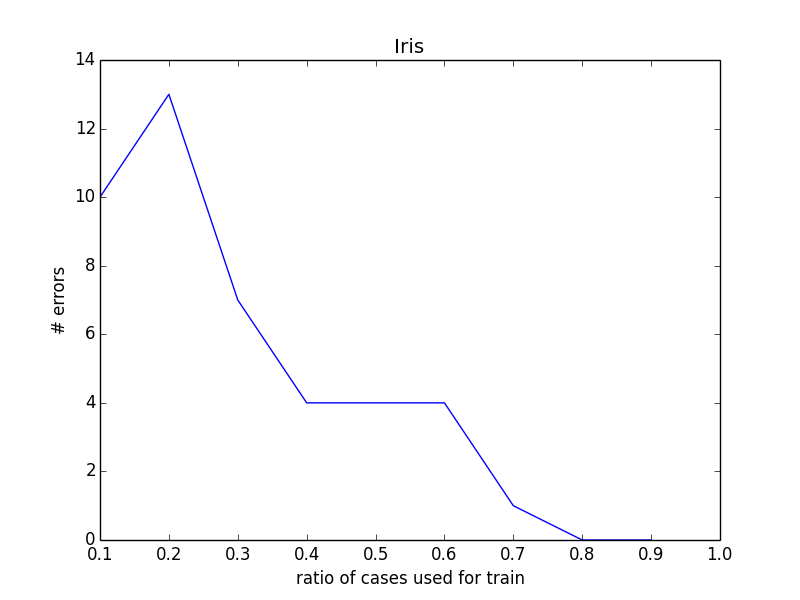
\includegraphics[width=0.7\linewidth]{images/iris}
    \caption{Iris}
    \label{fig:iris}
\end{figure}

\begin{figure}[htb]
    \center
    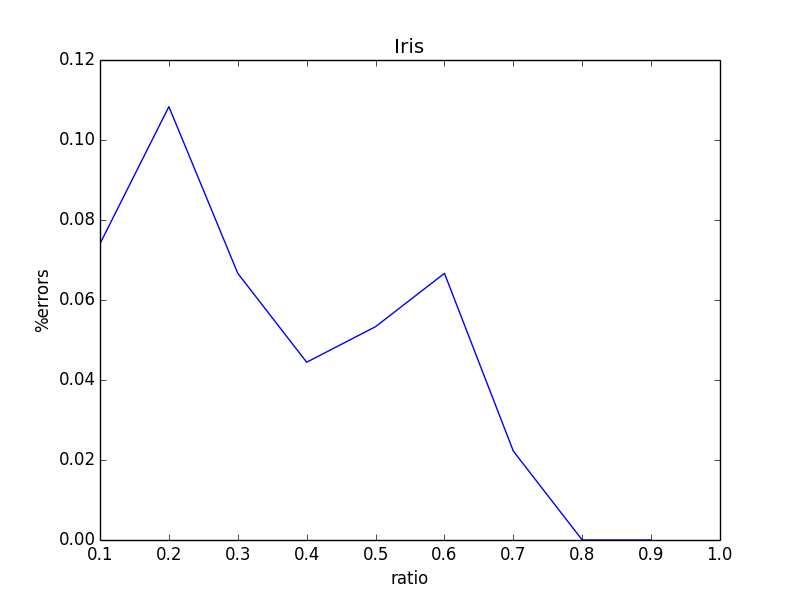
\includegraphics[width=0.7\linewidth]{images/iris_p_bo}
    \caption{Iris}
    \label{fig:irisp}
\end{figure}

In Figure \ref{fig:iris} and Figure \ref{fig:irisp} we can see how the errors predicting the class behaves in function of the ratio. The iris dataset contains $150$ items. Hence, if the ratio is $0.1$ the training set will have $15$ items while the test set $135$. While in Figure \ref{fig:iris} we show the number of errors in Figure \ref{fig:irisp} we take into account the amount of cases that falls into each dataset and outlines the percentatge of errors instead of the number of errors.

This charts allows the user to use the best setting. Moreover, we can observe that the results are good, even with a very short ratio of the instances we can predict with a 90\% of accuracy

Furthermore we also tested the titanic dataset. The procedure was the same but in this case we give to the CBR the structure of this dataset (without changing the code). Figure \ref{fig:t} and Figure \ref{fig:tp} shows the corresponding charts.

\begin{figure}[htb]
    \center
    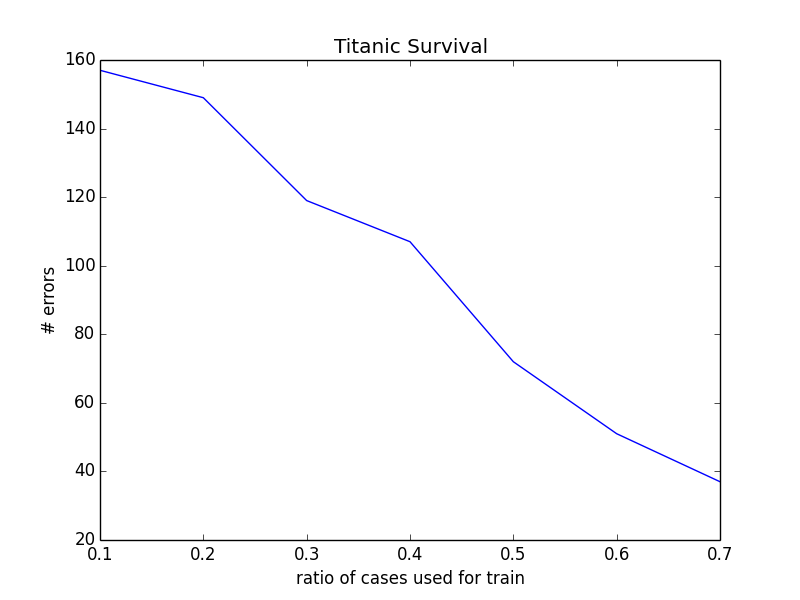
\includegraphics[width=0.7\linewidth]{images/titanic}
    \caption{Titanic}
    \label{fig:t}
\end{figure}

\begin{figure}[htb]
    \center
    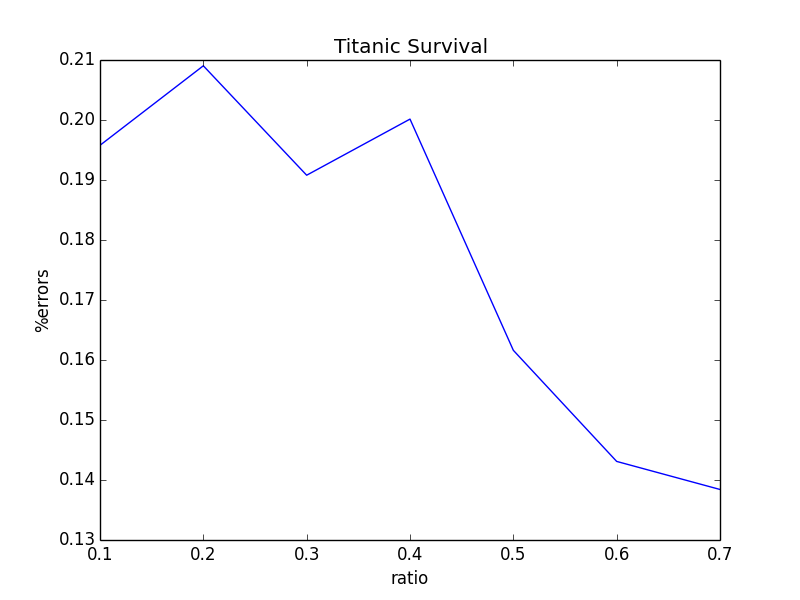
\includegraphics[width=0.7\linewidth]{images/titanic_p_bo}
    \caption{Titanic}
    \label{fig:tp}
\end{figure}

In the titanic case we have more instances ($891$) and each instance is more complex (it have more attributes and also more heterogeneous). In this case, hence, we infer that for this dataset we need a bigger ammount of cases stored in the case library in order reach better accuracy.

In Figures \ref{fig:iris},\ref{fig:irisp},\ref{fig:t},\ref{fig:tp} the $K$ parameter was fixed to 5. However, we can play, among others, with this parameters. For example, Figure \ref{fig:tk} and \ref{fig:tkp} draw the same Titanic results but executed with $K$ equal to 10 where we can see that we obtain a small improvement. Hence, by testing the dataset we can tune the settings in order to obtain better performance.


\begin{figure}[htb]
    \center
    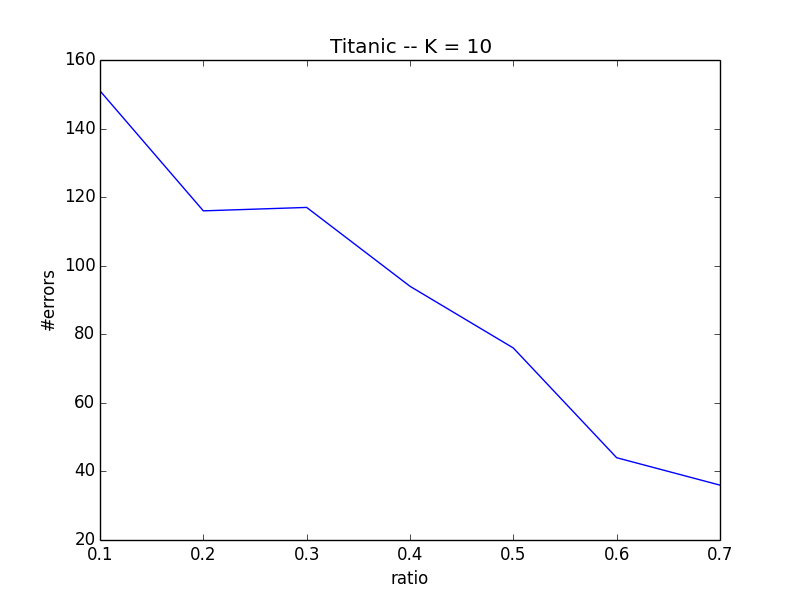
\includegraphics[width=0.7\linewidth]{images/tk10}
    \caption{Titanic}
    \label{fig:tk}
\end{figure}

\begin{figure}[htb]
    \center
    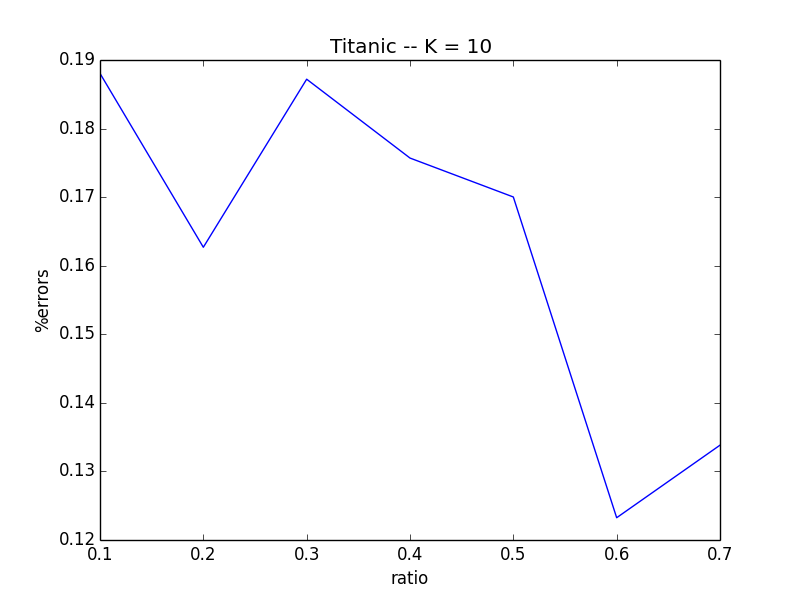
\includegraphics[width=0.7\linewidth]{images/tk10_p_bo}
    \caption{Titanic}
    \label{fig:tkp}
\end{figure}

\subsection{Files}

The files implemented are listed here:
\begin{itemize}
    \item \begin{description}
            \item[CBR.py] This file implements the command-shell interface that allows the user to interact with the CBR.
        \end{description}
    \item \begin{description}
            \item[flatMemory.py] Implementation of the flatMemory
        \end{description}
    \item \begin{description}
            \item[kdTree.py] Implementation of the kdTree
        \end{description}
    \item \begin{description}
            \item[Case.py] Implementation of a Case
        \end{description}
    \item \begin{description}
            \item[Attributes.py] Implementation of an Attribute
        \end{description}
    \item \begin{description}
            \item[CBRFunctions.py] Implementation of general functions that can be consumed by the others classes
        \end{description}
    \item \begin{description}
            \item[CBRTests.py] Implementation of the tests
        \end{description}
    \item \begin{description}
            \item[readingCsv.py] Implementation of the functions needed to read and format a csv file
        \end{description}


\end{itemize}

\section{Conclusion and Future work}

We built an interactive CBR that allows the user to execute it with any dataset since it can provide the structure by calling the implemented functions. It is programmed taking care about modularity, scalability and extensibility. With that characteristics it is quite straightforward to add new similarity functions of a particular kind of attribute without mesh up the rest of the processes, we only need to add the function and the program will handle it.

As a future work, we started an implementation aiming to accept a list as a kind of attribute. We had to rollback in order to have a working version for delivering. However, we want to remark the code is thought to incorporate this feature.

We believe that the incorporation of the list as a kind of attribute and consequently nested attributes will generate an exceptional generality. This is because we will be able to select lists as a solution (being able to recommend any kind of structure) covering different CBR tasks with a general model or have lists of lists of attributes wining a huge versatility or both.


\end{document}


